
\chapter{Introduction}\label{CAPINTRO}

Sexually Transmitted Diseases (STD) have been a major public health threat for a long time in human history. Modern concerns about STD began with the pandemic of syphilis which spread over Europe in the early sixteenth century. 

Human Papillomavirus (HPV) is the most common STD. It is transmitted via vaginal, anal, or oral sex with someone who has the virus \cite{CDC_VPH}. Persistent HPV infections with genotypes 16 and 18 are responsible for about $70\%$ of all cervical cancer, with $40-85\%$ of other anogenital cancers and also $16-28\%$ of the head and neck cancers. Furthermore, HPV is a cause of other non malignant diseases, to mention genotypes 6 and 11 cause about $90\%$ of anogenital warts, and secondarily juvenile onset of recurrent respiratory papillomatosis \cite{castellsague2012prevalence}.

Most of the modeling approaches to STD in general and HPV in particular are done using classical models where the hypothesis of homogeneous mixing (everybody can transmit a disease to everybody) is implicitly assumed. However, when STDs are considered, homogeneous mixing is not a reasonable hypothesis and consequences of this assumption can be seen, for instance, in that the effects of vaccination schedules against HPV have been detected much sooner than what the models predicted \cite{fairley2009}.

Therefore, the structure and properties of networks of sexual contacts in human populations and the building of reliable sexual partner networks, as in \cite{NOVA_LSP}, is a public health topic of key interest in connection with the spread of STD. However, this problem has received scarce attention in the world of computational modeling and the modeling of STD epidemiology is usually based upon theoretical proposals in terms of the network structure. 

In the last years, we have been working on modeling the dynamics of several phenomena using large random networks \cite{acedo2011using,acedo2015firing,gonzalez2015modelling} and we know that, under this approach, it is necessary to perform a lot of simulations for model calibration. To do so, a distributed computing environment called \textit{Sisifo} \cite{wiki_sisifo} was developed \cite{villanueva2013epidemic}. Using this environment we were able to find, using exhaustive searching, model parameters that made the model output close to given data, that is, calibration. 

The next step was to find out how to reduce the number of simulations studying the inclusion of optimization algorithms. In \cite{cortes2016modeling} we presented  an attempt with small networks and in an only computer. 

Then, in this paper, we describe how to adapt the optimization algorithm named Particle Swarm Optimization (PSO) in the distributed computing environment \textit{Sisifo} to calibrate a large network of lifetime sexual partners (LSP) where we want to study the transmission dynamics of two types of HPV: the high and the low risk. High risk HPV gathers the types of HPV related to the apparition of precancerous lesions or cancers. Low risk HPV types are the ones that can develop genital warts.

This paper is organized as follows. In Section 2 we give an overview of the LSP network building and describe the transmission dynamics of both types of HPV on LSP networks. In Section 3, we summarize the functioning of the distributed computing environment \textit{Sisifo}. Also, we describe how to incorporate and adapt the PSO algorithm to this environment. In Section 4 we present the results and, finally, in Section 5, conclusions are discussed.  

\section{HPV network model building}
Here we give a general review of the method presented in \cite{NOVA_LSP} where an algorithm to build LSP networks consistent with the distribution of the number of partners for both males and females reported in the Health and Sexual Habits Survey in Spain \cite{INE}, has been described. Then, on the LSP networks, we will define the transmission dynamics of high and low risk HPV.

First, we consider the population of the Community of Valencia (Spain) \cite{CV_wiki} and its demographic structure \cite{pegv} given in Figure \ref{demog}, where we show the number of men and woman per age.

\begin{figure}[h]
	\centering
	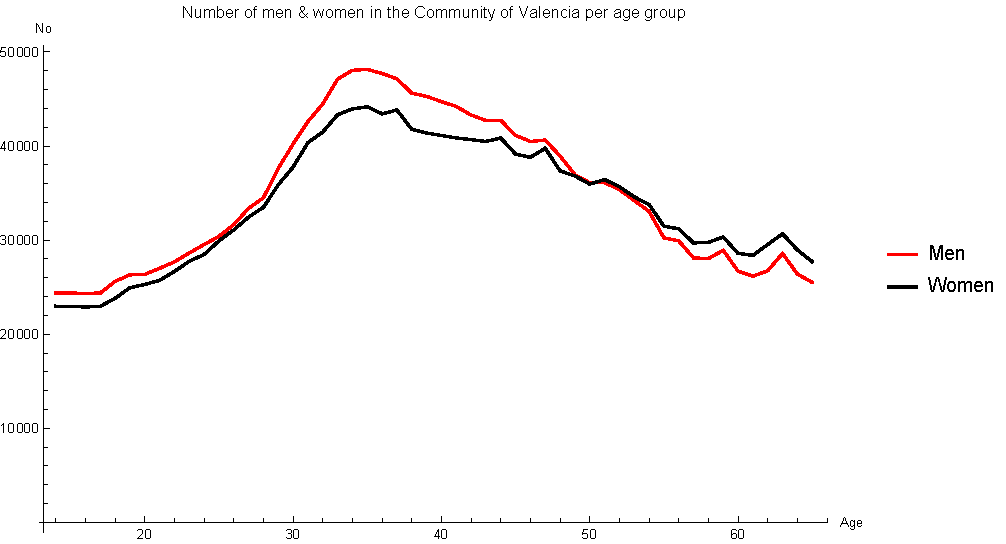
\includegraphics[scale=0.6]{demog.pdf}
	\caption{Number of men and woman in the Community of Valencia per age (year 2013).}
	\label{demog}
\end{figure}

Now, we consider data about the lifetime sexual partners for both males and females reported in the Health and Sexual Habits Survey in Spain \cite{INE} as can be seen in Figure \ref{lsp}. The asymmetry in the behavior of males and females have to be taken into account in the construction of the network.

\begin{figure}[h]
	\centering
	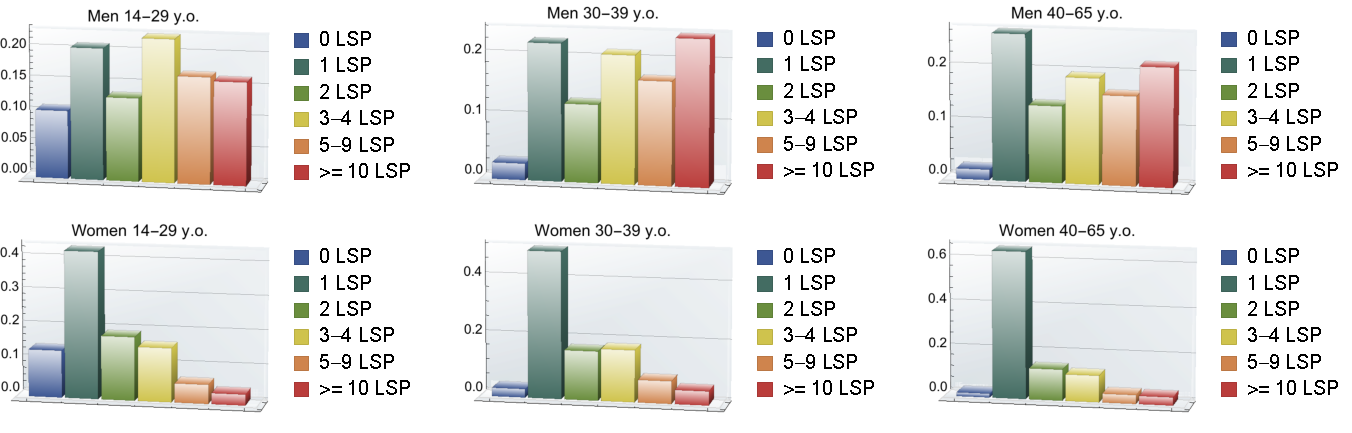
\includegraphics[scale=0.5]{lsp.pdf}
	\caption{Number of lifetime sexual partners (LSP) for men and woman per age group in Spain (year 2003). The age groups are 14-29, 30-39 and 40-65.}
	\label{lsp}
\end{figure}

The estimated percentage of homosexual men is $3.88\%$ \cite{INE}. The situation for the homosexual men population is different of the one shown in Figure \ref{lsp}, because the average number of sexual partners is estimated in 39 regardless of age, but this number increases with age with a peak of 59 in the 40-49 age-group \cite{Durex2002}. 

A difficulty arises because we have little information about the number of sexual contacts in homosexual women subpopulation. In a personal communication by Dr. Mireia Díaz from the Catalan Institute of Oncology (IDIBELL) we were informed that HPV hardly spreads among homosexual women, and almost all homosexual men, sometimes in their lives, had a woman partner. Consequently, we have simulated these connections by assigning a contact to every man in the homosexual subpopulation with woman with 5 partners or more. This is done according to the assortativity principle, that is, people use to join with people with similar habits.

Taking into account the above premises, for the average number of LSP of men $k$ and for each one of the $N$ individuals (nodes) in the network

\begin{enumerate}
	\item Using the demographical information, we assign randomly the sex (man/woman) and age.
	\item We label $3.88\%$ of men as homosexual men, randomly.
	\item Depending on the age and gender, and using the data about LSP for men and women, we assign randomly the number of LSP he/she is going to have.
	\item We assign randomly LSP to homosexual men depending on their age following the report \cite{Durex2002}.
\end{enumerate}

The above algorithm determines the sex, age and number of LSP of each node. Now, we have to build the network that matches with the LSP of the nodes. 

\begin{enumerate}
	\item Separate men and women nodes into two groups.
	\item Order women in descendant order of LSP.
	\item For each woman node:
	\begin{enumerate}
		\item we pair her with as much heterosexual men as the number of LSP she has. Among all the possibilities to pair we try to choose those men with similar number of LSP. 
	\end{enumerate} 
	\item For each homosexual men node:
	\begin{enumerate}
		\item we pair him with as much homosexual men as the number of LSP he has.
		\item Assign to every homosexual men a woman with $5$ partners or more. 
	\end{enumerate} 
\end{enumerate}

The procedure to pair heterosexual partners is the same we use to pair homosexual partners. In Figure \ref{red} we can see a small LSP network. Details about how to build the heterosexual networks can be found in \cite{NOVA_LSP}. 

\begin{figure}[h]
	\centering
	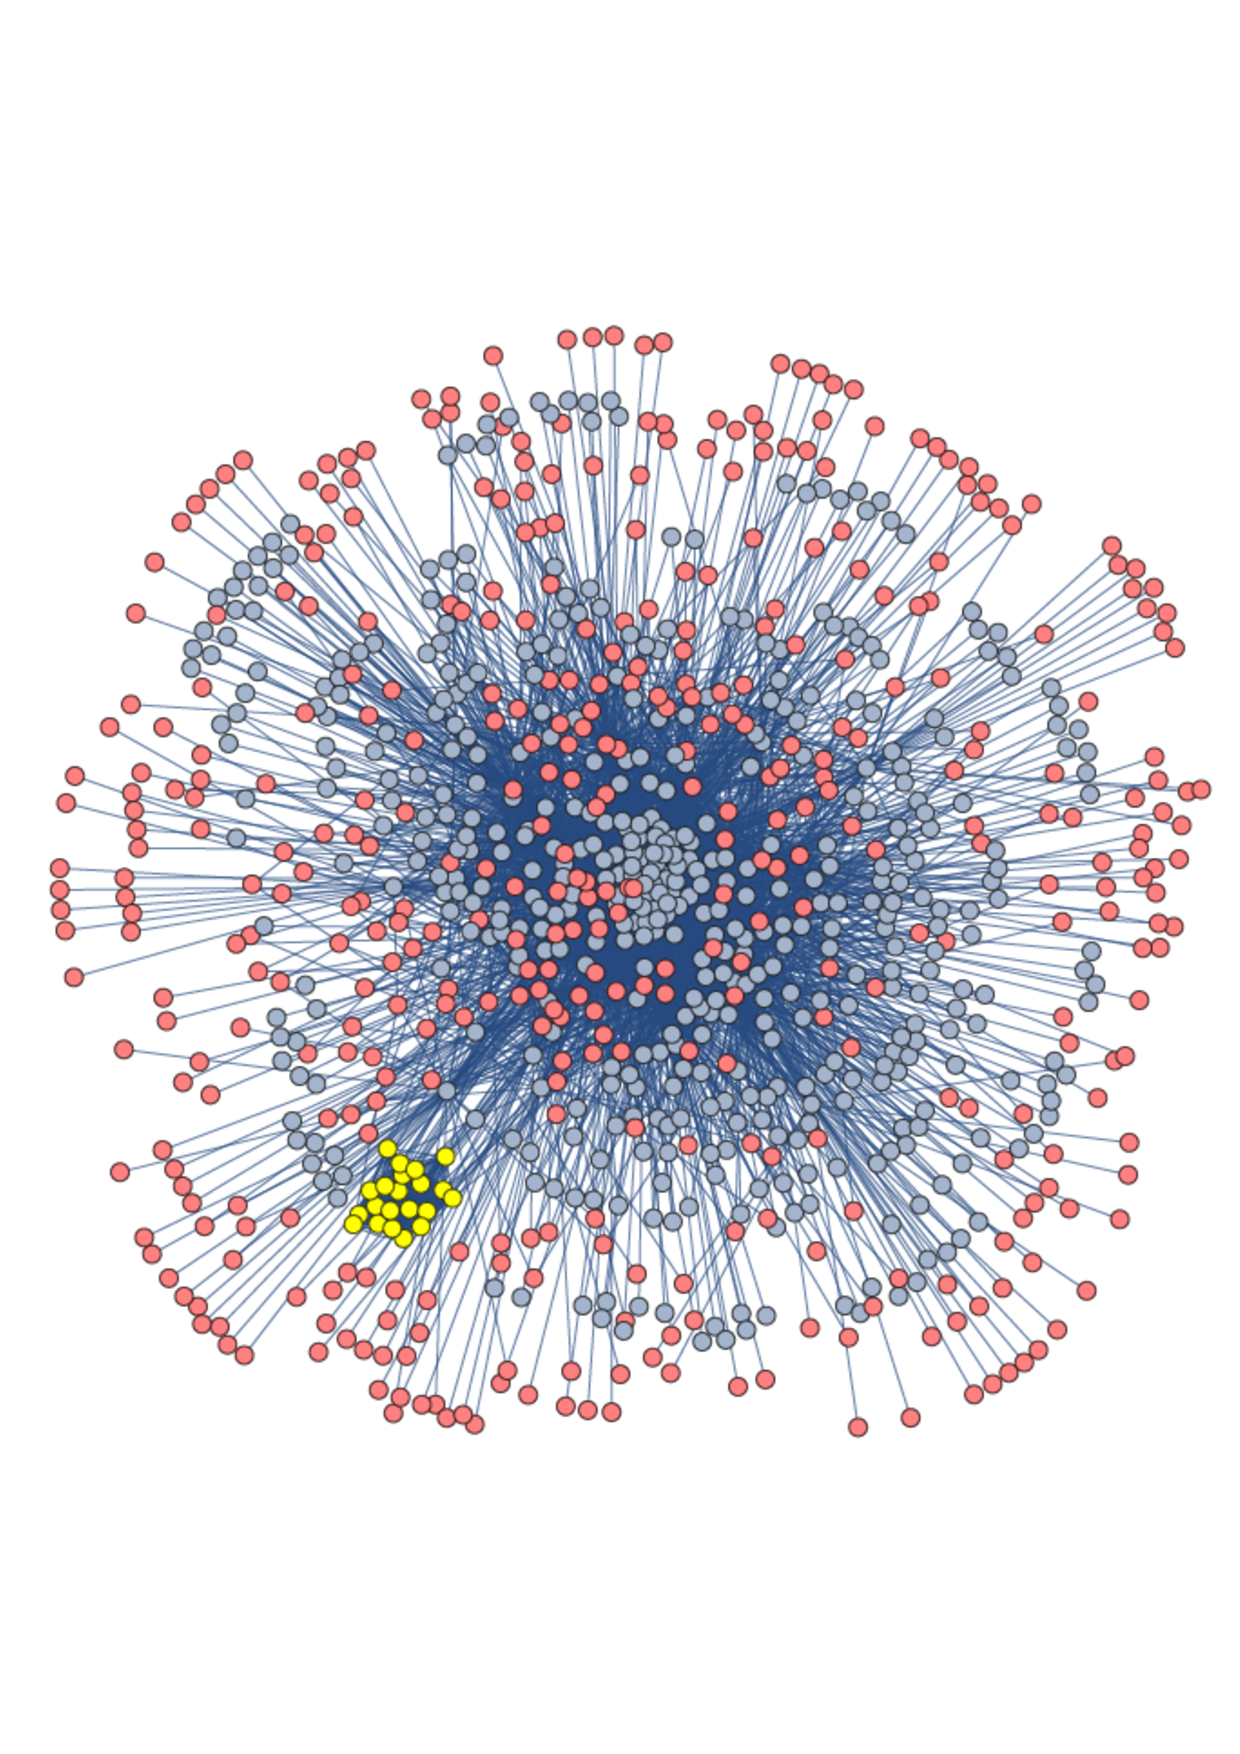
\includegraphics[scale=0.4]{red.pdf}
	\caption{LSP network for 1000 individuals: blue dots correspond to men, pink to women and yellow to homosexual men.}
	\label{red}
\end{figure}

\subsection{HPV prevalence data}
Data provided by \cite{castellsague2012prevalence} allow us to determine an estimation of the prevalence of the HPV. Then, we divide the data of infectious women into the age groups $18-29$, $30-39$ and $40-65$, the same age groups as those given by the Sexual Behaviour Habits Survey \cite{INE} and used to build the LSP networks. 

Taking into account that an infected individual with high risk HPV may develop precancerous lesions and, eventually, cancer, and that an infected individual with low risk HPV may develop genital warts, we say that an individual is HR-infected if he/she has been infected by a high risk HPV. That individual may also be infected by a low risk HPV (co-infection). Analogously, an individual is LR-infected if he/she has been infected by a low risk HPV. That individual may also be infected by a high risk HPV (co-infection). Then, the percentage of women HR- and LR-infected per the aforementioned group ages, are collected in Table \ref{datos}. 

\begin{table}[h]
	\small\sf\centering
	\caption{Prevalence of HR- and LR-infected women per age groups. Mean and $95\%$ confidence intervals.}
	\begin{tabular}{c|ccc}
		\toprule
		Women & HR-infected & LR-infected \\
		\midrule
		$18-29$ y.o. & $24.10\%$, $[21.33\%, 26.98\%]$ & $6.36\%$, $[4.71\%, 8.07\%]$ \\
		$30-39$ y.o. & $11.01\%$, $[7.54\%, 15.09\%]$ & $1.26\%$, $[0.0\%, 3.14\%]$ \\
		$40-64$ y.o. & $5.96\%$, $[4.29\%, 7.8\%]$ & $2.37\%$, $[1.22\%, 3.68\%]$ \\
		\midrule
		$18-64$ y.o. & $16.23\%$,$[14.52\%, 17.97\%]$ & $4.41\%$, $[3.42\%, 5.45\%]$ \\
		\bottomrule
	\end{tabular}
	\label{datos}
\end{table}

\subsection{HPV dynamics on a LSP network}
Over the LSP networks, we introduce the transmission dynamics of the HPV. Thus, non-infected individuals may get infected if they have sexual intercourses with HR- or LR-infected sexual partners. Being infected, the individuals may infect other susceptible sexual partners. After a period of time depending on the type of infection (HR or LR), the individuals recover and move from the contagious state to susceptible state, clearing the infection.

The above description leads to consider the following model parameters that determine the model behavior. These parameters are:

\begin{itemize}
	\item Global probabilities in order to determine if a LSP produces a contagion in the current time step per age group $14-17$, $18-29$, $30-39$ and $40-65$. Taking into account that the edges that represent LSP are fixed and permanent, we need to modulate the possibility of contagion in a certain period. Then, we include the model parameters $T_0, T_1, T_2$ and $T_3$ to modulate these contagion in every month for group ages $14-17$, $18-29$, $30-39$ and $40-65$, respectively (4 parameters).
	\item Average time an individual infected by a high (low) risk HPV clears the infection and recovers (2 parameters).
	\item Probability that a woman (man) infected of high (low) risk HPV transmits it to his/her
	partner in a sexual intercourse (4 parameters). 
\end{itemize}

Also, we should recall that, for LSP network building, we need to provide the average number of men LSP $k$. Then, we have a total of 11 model parameters to be determined.

For the simulations we are going to show hereinafter, the networks will have $200\ 000$ nodes and the temporal step used is defined as a month.

Hence, we have implemented in C++ a simulator that, given the above described model parameters, it builds a LSP network and performs a simulation of the transmission dynamics of high and low risk HPV. 

Note that the transmission parameters involve certain probabilities. Then, in order to see if a contagion has been carried out by a sexual intercourse, we simulate this by generating a random number and checking if it is less than the corresponding threshold given by the model transmission parameters. Therefore, the randomness is included into the model in a natural way producing some uncertainty on the model output that has to be quantified.

After all the above considerations, now, the goal is, assuming that we are in a stable situation, to calibrate the model parameters in such a way that the model output related to women HR and LR prevalence is as close as possible to the data in Table \ref{datos}.
